\subsection{Results and Analysis} \label{Result section}
\todo{This section needs update.}
\subsubsection{Sampling Gradients results}
Table \ref{Experiment summary table} states all the combinations of ansatzes and methods.

The ansatz gradient variances decay as expected for the unrestricted setting.
The decay rate is exponentially fitted with the rate of -0.63.
The figure \ref{Plot ansatzes variance}a shows the results of the ansatz in this configuration.
The semi-log plots portray the variances of gradient from the ansatz in the unrestricted configuration.
Consider that the unit measure for variance is in \emph{exponential} form, so the linear graph is exponentially closer to zero for each qubit added to the circuit.
This result indicates that the cost function landscape becomes flatter and flatter.
Eventually, the gradient would reach a near-zero value across a large plateau, which would be inefficient for any gradient-based optimization algorithm to train the model.
We discussed this phenomenon in Section \ref{Barren Plateaus section}.


\begin{figure}
    \centering
    \begin{subfigure}[b]{.49\textwidth}
        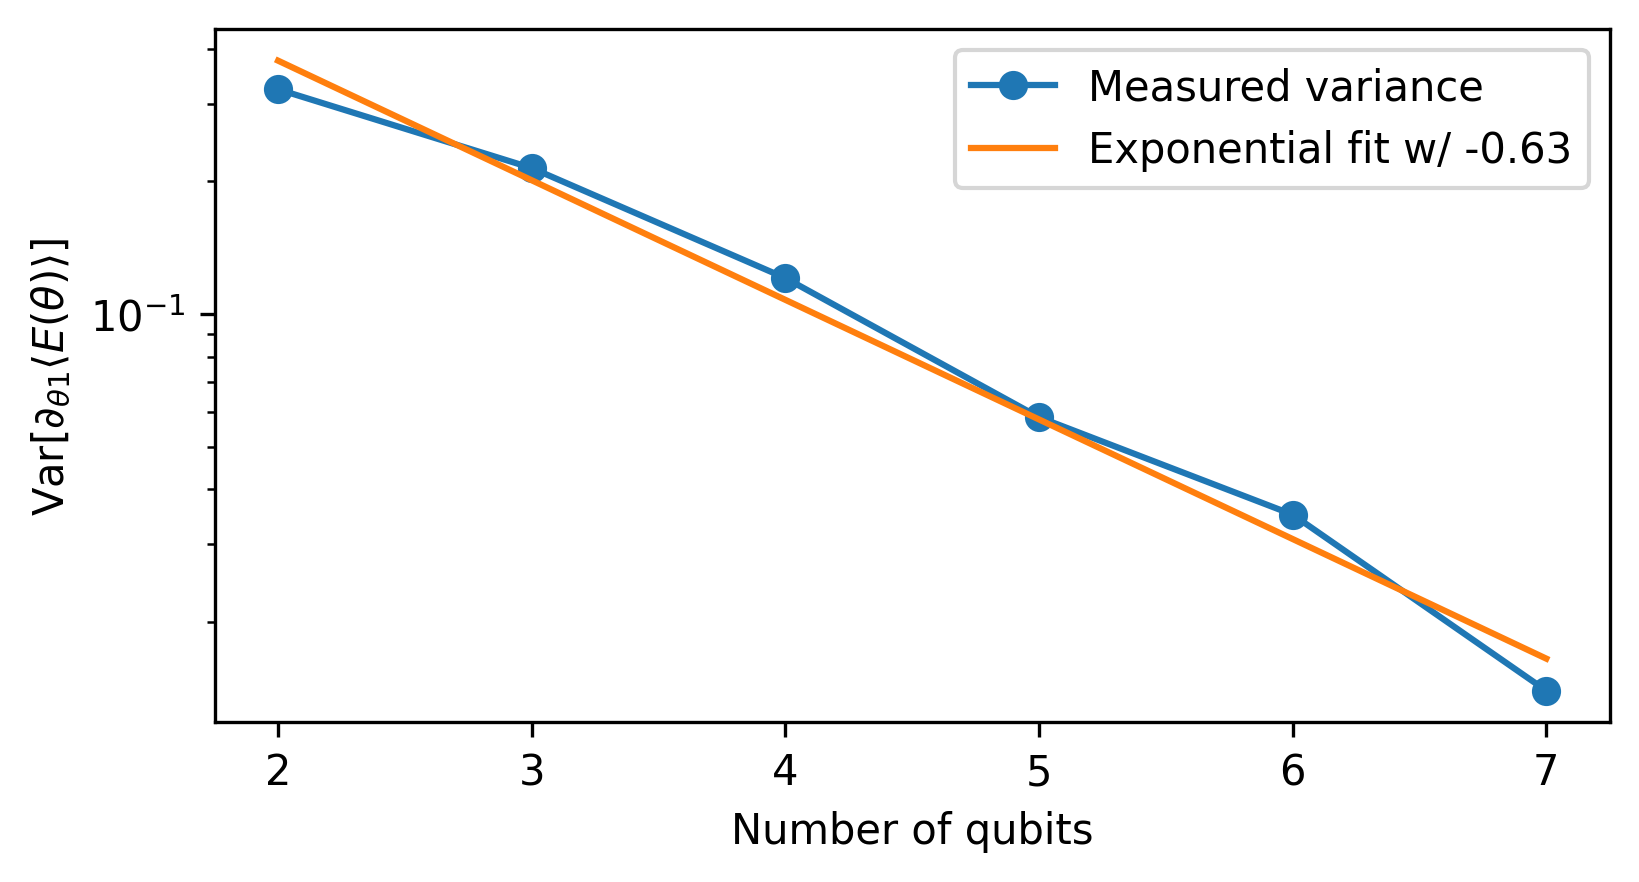
\includegraphics[width=\textwidth]{Artefact/Appendices/var0.png}
        \centerline{a) Method \#0 variances}
    \end{subfigure}
    \hfill
    \begin{subfigure}[b]{.49\textwidth}
        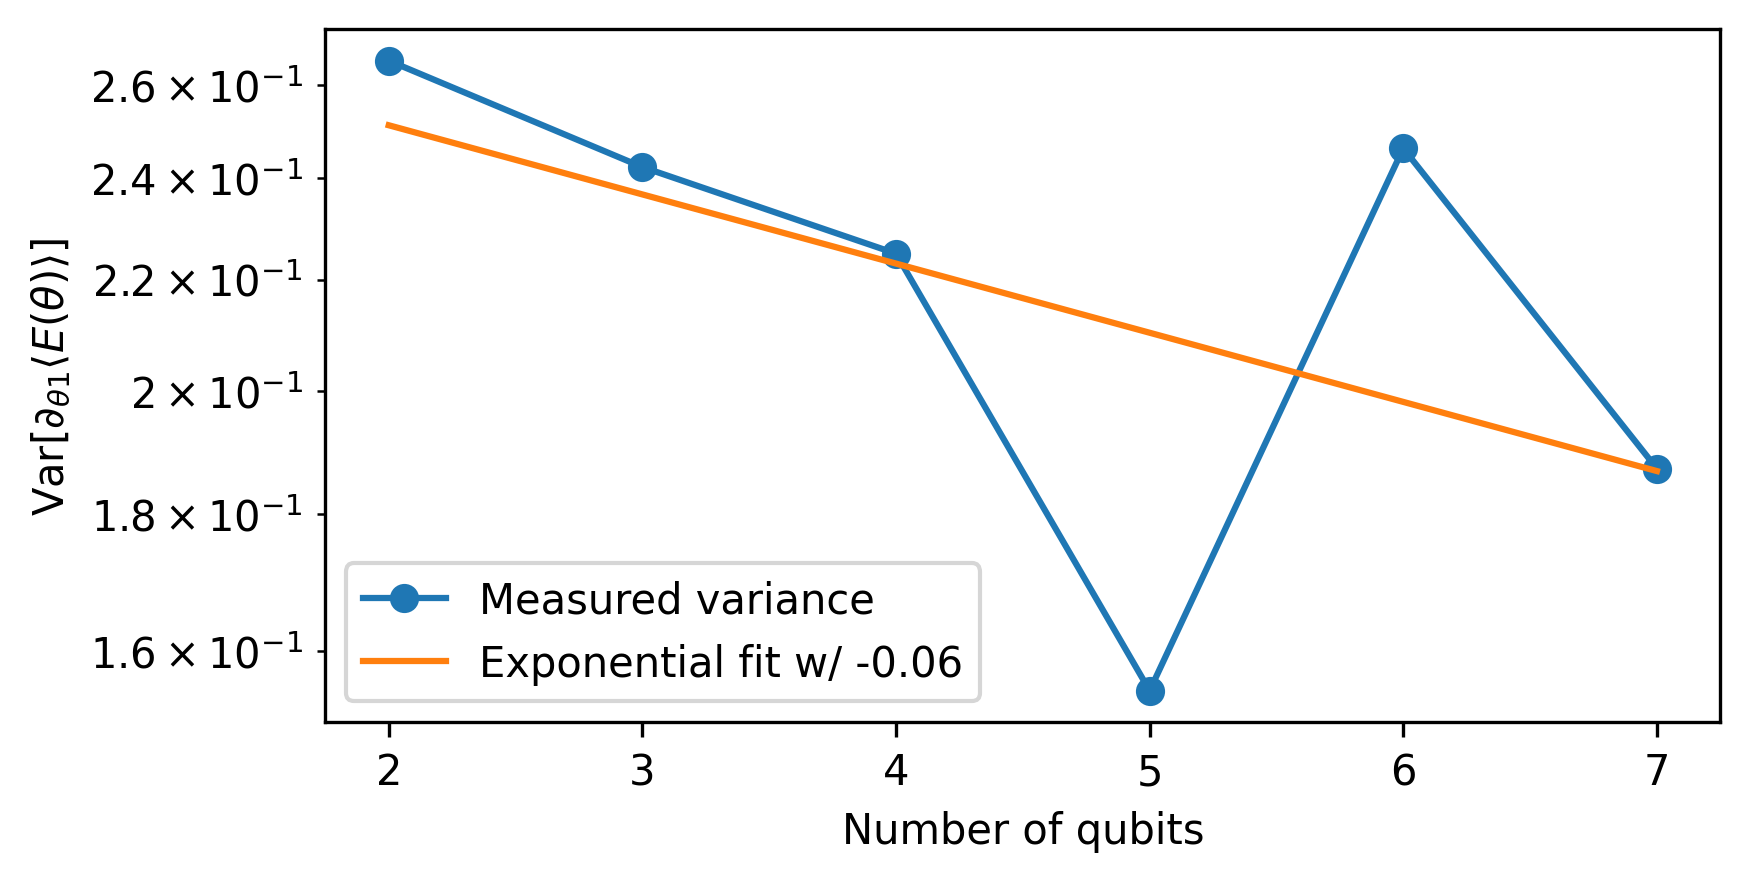
\includegraphics[width=\textwidth]{Artefact/Appendices/var1.png}
        \centerline{b) Method \#1 variances}
    \end{subfigure}

    \begin{subfigure}[b]{.49\textwidth}
        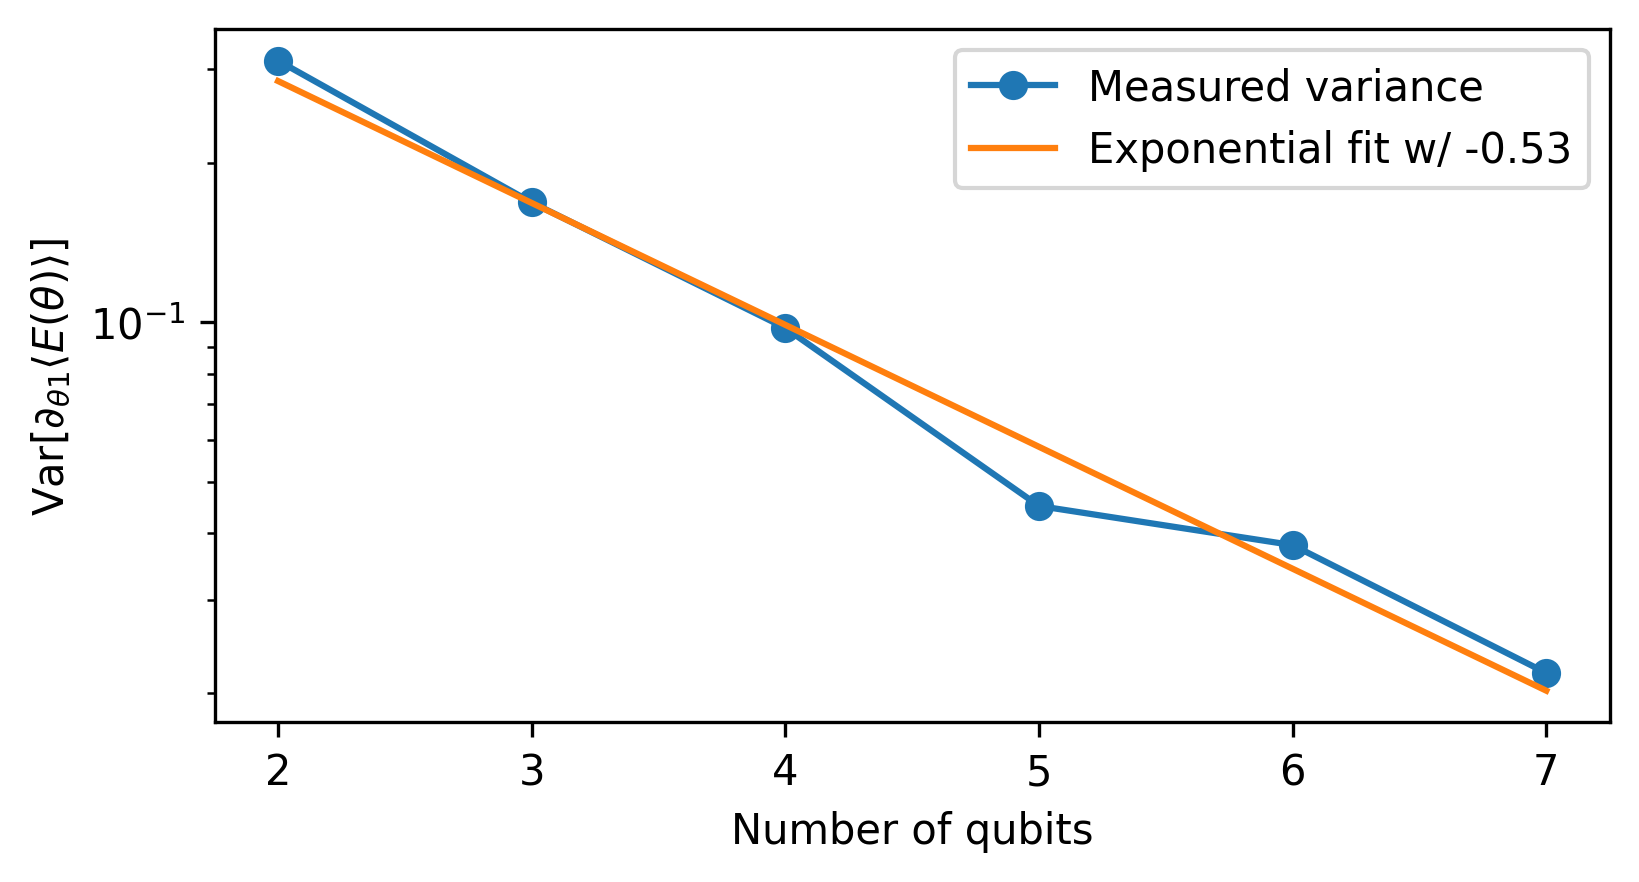
\includegraphics[width=\textwidth]{Artefact/Appendices/var2.png}
        \centerline{c) Method \#2 variances}
    \end{subfigure}
    \hfill
    \begin{subfigure}[b]{.49\textwidth}
        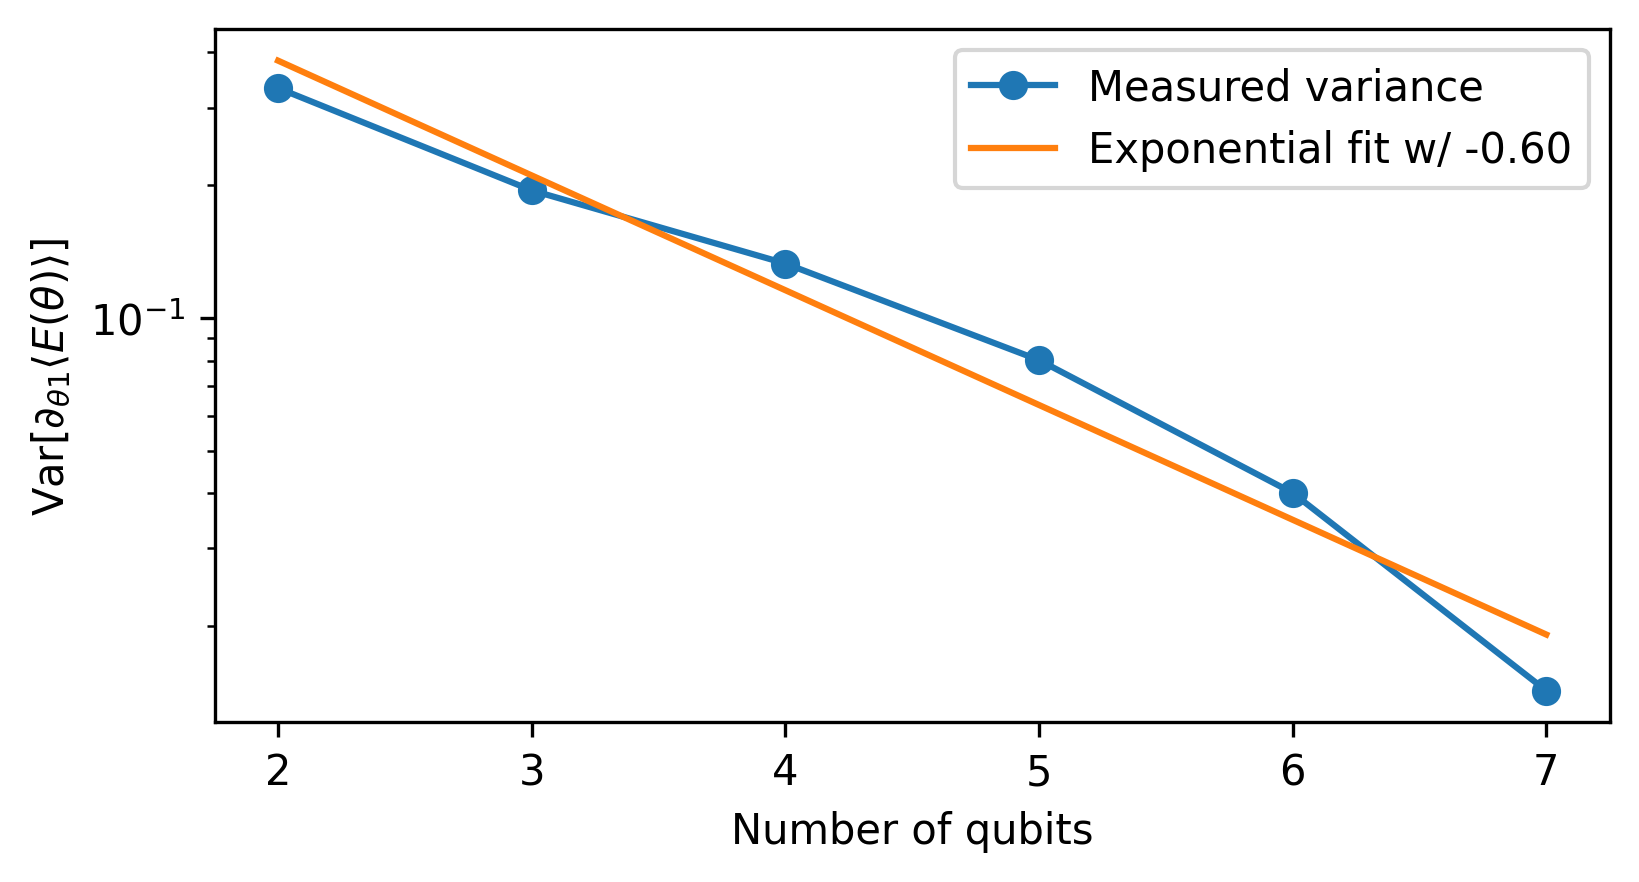
\includegraphics[width=\textwidth]{Artefact/Appendices/var3.png}
        \centerline{d) Method \#3 variances}
    \end{subfigure}

    \caption{
        The variances of gradient from differences ansatzes in the four configurations.
        For each iteration, we increase the qubit and repetition count by 1, starting from 2 to 7.
        The variances vanish exponentially to the number of qubits.
        For method\#1, we keep the repetition value fixed as 1.
    }
    \label{Plot ansatzes variance}
\end{figure}

In contrast, for the case of Local Cost Function and Shallow circuit, we observe that the variances of the ansatz' gradient did not vanish when we attempted to increase the number of qubits.
The slope of the ansat in this case decay exponentially fit with -0.06.
This implies that the cost function landscape can sustain the slope.
Figure \ref{Plot ansatzes variance}b shows the result of the experiment for local cost function and shallow circuit.
We can see that the ansatz produced an unstable graph which mean the trainability of gradient-based optimization algorithms would not be consistent.
For example, the variance value for 6 qubits is higher compared to 3, 4 or 5 qubits.

To compare the effectiveness of the local cost function treatment, we plot the variance graph of above mention cases in Figure \ref{Plot variance default and Local Cost} and the Table \ref{Experiment summary table}.
The results have shown the differences in the decay rates of different ansatzes and methods.
Overall, the ansatzes with the local cost function and restriction on circuit depth have their variance values remaining higher and being more consistent for higher qubit count.
The ansatz with this treatment, therefore would not possess a barren plateau.
On the other hand, the values for the default cases shrink exponentially and eventually, the near-zero gradient around the initial point will expand to a large plateau.



\begin{figure}
    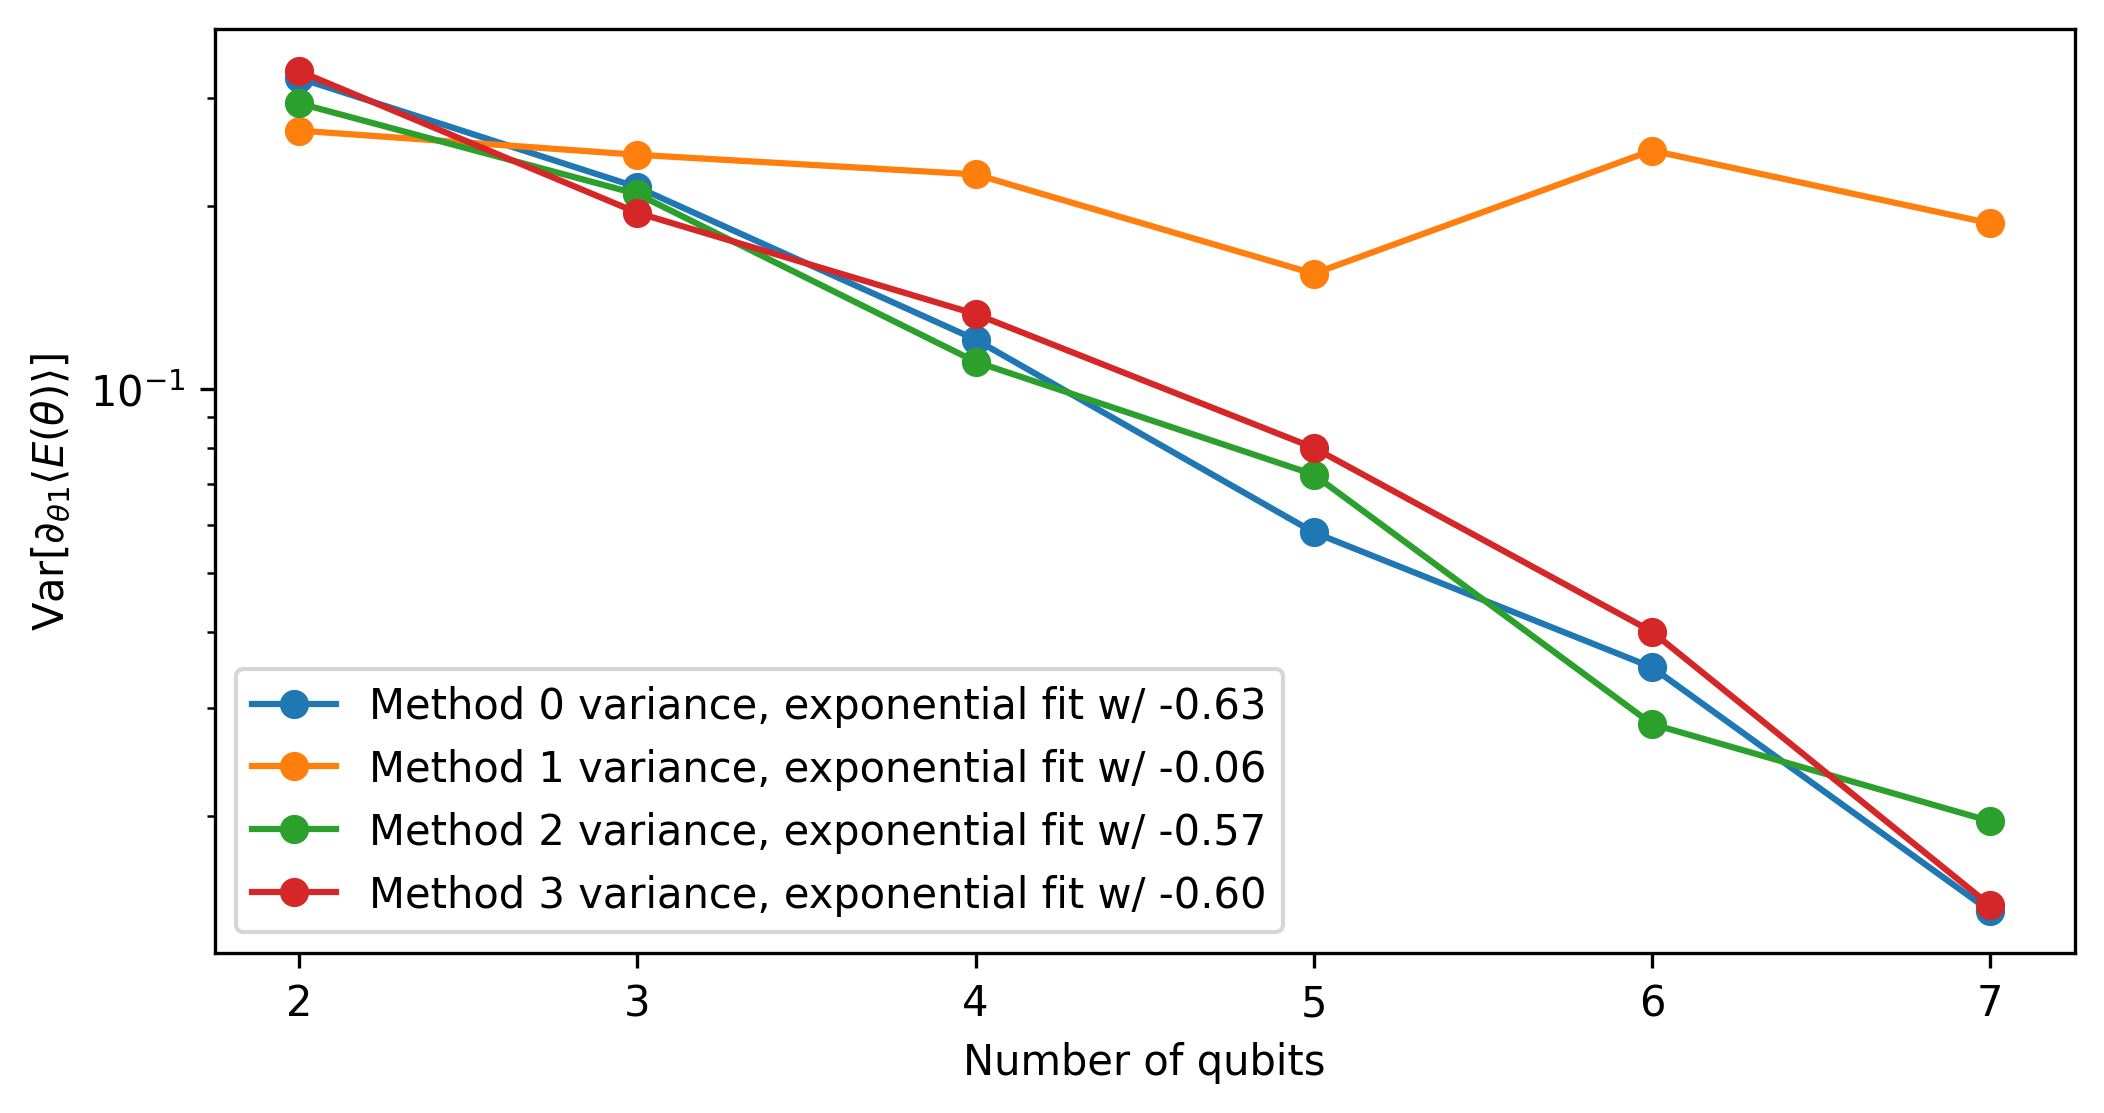
\includegraphics[width=\textwidth]{Artefact/Appendices/variances.png}
    \caption{
        Comparison of the variance values of the ansatzes with four treatments applies.
        The ansatz with local cost function and fixed depth has its variance decay at a significantly smaller rate (-0.06) compared to the rest.
    }
    \label{Plot variance default and Local Cost}
\end{figure}


\subsubsection{Classification Results}